\documentclass[12pt,a4paper]{article}
\usepackage[utf8]{inputenc} %polskie znaki
\usepackage[T1]{fontenc}	%polskie znaki
\usepackage{amsmath}		%matematyczne znaczki :3
\usepackage{enumerate}		%Dodatkowe opcje do funkcji enumerate
\usepackage{geometry} 		%Ustawianie marginesow
\usepackage{graphicx}		%Grafika
\usepackage{wrapfig}		%Grafika obok textu
\usepackage{float}			%Allows H in fugire
%\pagestyle{empty} 			%usuwa nr strony

\newgeometry{tmargin=2cm, bmargin=2cm, lmargin=2cm, rmargin=2cm} 

\begin{document}
	\begin{center}
		\LARGE Rachunek Prawdopodobieństwa - część 2
	\end{center}
	\vspace{1cm}
	\begin{enumerate}[1.]
		\item W urnie jest 20 kul ponumerowanych od 1 do 20. Wyjmujemy losowo jedną kulę. Oblicz prawdopodobieństwo, że numer na wylosowanej kuli będzie:
		\begin{enumerate}[a)]
			\item większy od 8
			\item podzielny przez 5
			\item liczbą pierwszą
		\end{enumerate}
	\item W pierwszej urnie są 2 kule białe i 4 kule czarne. W drugiej jest 1 kula biała i 4 kule czarne. Z każdej urny wyciągamy po jednej kuli. Oblicz prawdopodobieństwo, że wylosowane kule będą tego samego koloru.
	\item Oblicz prawdopodobieństwo, że w trzech rzutach symetryczną kostką sześcienną do gry suma kwadratów liczb uzyskanych oczek będzie podzielna przez 3.
	\item W pierwszej urnie są 3 kule białe, 2 czarne i 4 zielone. W drugiej urnie są 4 białe, 5 czarnych i 1 zielona. Losowanie polega na rzuceniu symetryczną monetą i jeśli wypadnie orzeł to losujemy z pierwszej urny, jeśli reszka to z drugiej urny. Oblicz prawdopodobieństwo wylowania kuli
	\begin{enumerate}[a)]
		\item białej
		\item czarnej
		\item zielonej
	\end{enumerate}

	\item Na sali jest 12 ławek w 4 rzędach. 12 uczniów losuje miejsca na sali. Jakie jest prawdopodobieńostwo, że studenci A, B i C będą siedzieli w tym samym rzędzie?
	
	\item Trzy osoby wsiadają losowo do pociągu, składającego się z 5 wagonów. Jakie jest prawdopodobieńostwo, że każda z tych osób odbędzie podróż w innym wagonie?
	
	\item Jakie jest prawdopodobieńostwo, że w losowo wybranej grupie 23 osób, znajdą się co najmniej dwie, które obchodzą urodziny tego samego dnia?
	
	\item W pudełku A znajduje się 5 kul białych i 7 kul czarnych. Wybieramy losowo jedną kulę. Jeżeli wylosujemy kulę białą losujemy ponownie jedną kulę z tego pudełka, a jeżeli wylosowaliśmy kulę czarną, losujemy jedną kulę z pudełka B, w którym znajduje się 7 kul białych i 8 kul czarnych. Jakie jest prawdopodobieńostwo, że w drugim losowaniu wybierzemy kulę białą?
	
	\item Dziecko bawi się literkami A, A, A, E, K, M, M, T, T, Y . Oblicz prawdopodobieństwo, że przypadkowo złoży
	ono słowo MATEMATYKA.
	
	\item W szafie jest 10 par butów. Losujemy 4 buty. Oblicz prawdopodobieństwo, że wylosujemy co najmniej jedną parę.
	
	\item W urnie jest 6 kul białych, 3 kule czarne i pewna liczba kul niebieskich. Oblicz ile jest kul niebieskich, jeżeli prawdopodobieństwo wylosowania kuli białej z tej urny wynosi $\frac{1}{3}$. 
	\end{enumerate}

\newpage

	\begin{center}
	\LARGE Statystyka
\end{center}
\vspace{1cm}
\begin{enumerate}[1.]
	\item Oblicz medianę i średnią arytmetyczną liczb: $\{2,\:4,\:5,\:3,\:7,\:9,\:-2\}$
	\item Średnia arytmetyczna liczb: $\{x,\:3,\:1,\:4,\:1,\:5,\:1,\:4,\:1,\:5\}$ jest równa 3. Oblicz "x".
	\item Poniższa tabela przedstawia wyniki sprawdzianu klasy IV
	
	\begin{tabular}{|c|c|c|c|c|c|c|}
		\hline
		Ocena&1&2&3&4&5&6\\
		\hline
		Liczba uczniów&2&4&5&6&2&1\\
		\hline
	\end{tabular}

Oblicz medianę, średnią arytmetyczną i dominantę tych ocen.

\item Średnia wieku w pewnej grupie studentów jest równa 23 lata. Średnia wieku tych studentów i ich opiekuna jest równa 24 lata. Opiekun ma 39 lat. Oblicz, ilu studentów jest w tej grupie.

\item Przeprowadzono badania, dotyczżce liczby osób jadżcych w samochodach osobowych w godzinach rannych, w kierunku centrum pewnego miasta. Wyniki badań przedstawione są na digramie kołowym.

\begin{figure}[h]
	\centering
	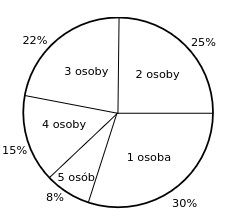
\includegraphics{stat1.jpeg}
\end{figure}
\begin{enumerate}[a)]
	\item Oblicz śrędnią liczbę osób jadących w samochodzie osobowym w godzinach rannych. Wyznacz również medianę i dominantę.
	\item Oblicz prawdopodobieństwo, że w losowo wybranym samochodzie osobowym, w godzinach
	rannych, w kierunku centrum, były więcej niż 3 osoby.
	\item Wiedząc, że samochodów osobowych, w których były 4 osoby, zaobserwowano o 350 więcej,	niż samochodów w których było 5 osób, oblicz, ile wszystkich samochodów obserwowano w
	trakcie badań.
\end{enumerate}
\end{enumerate}

\end{document}